\chapter{Miroirs et lentilles minces}\label{ch:b1:mirrors-thin-lenses}

Un miroir de maquillage montre un visage deux fois plus grand~; le dos
d'une cuillère le montre minuscule et droit, son creux minuscule et
renversé~; une loupe tenue à bout de bras met la pièce à l'envers, tenue
près de l'œil elle agrandit un timbre~; un objectif de téléphone gros
comme une \omterm{def:b1:mirrors-thin-lenses:lens}{lentille} peint toute la rue sur un capteur. Une seule relation
algébrique entre trois distances gouverne chacune de ces \omterm{def:b1:mirrors-thin-lenses:image}{images}, et ce
chapitre l'établit --- pour les miroirs courbes d'abord, puis pour la
\omterm{def:b1:mirrors-thin-lenses:lens}{lentille mince} dont presque tous les instruments d'optique sont faits.

\begin{omfigure}
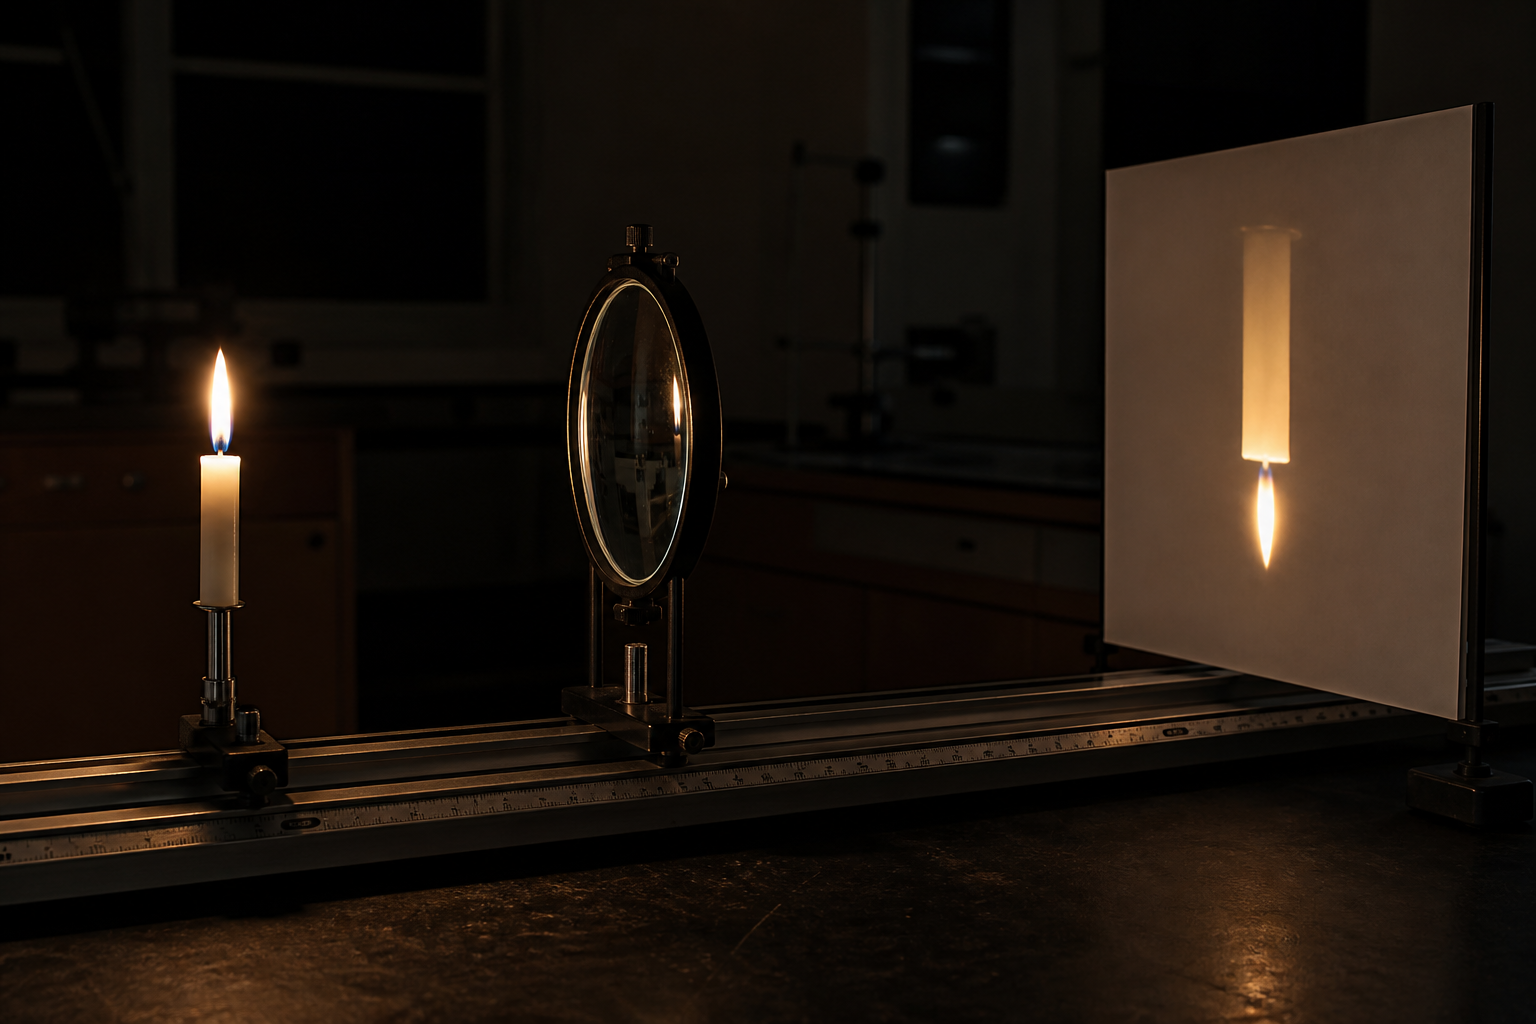
\includegraphics[width=0.60\linewidth]{images/book3/ai/b3-03-lens-candle-image.png}

{\small Une \omterm{def:b1:mirrors-thin-lenses:lens}{lentille convergente} forme sur un écran l'\omterm{def:b1:mirrors-thin-lenses:image}{image réelle} et renversée d'une flamme de bougie~: les distances de l'objet et de l'\omterm{def:b1:mirrors-thin-lenses:image}{image} obéissent à la relation de conjugaison de ce chapitre.}
\end{omfigure}

\section{Images et conditions de Gauss}

\begin{definition}[Objet, image, stigmatisme]\label{def:b1:mirrors-thin-lenses:image}
\index{image (optique)}\index{objet (optique)}\index{stigmatisme}\index{image réelle}\index{image virtuelle}
Un système optique reçoit les rayons issus d'un point $A$ (le
\emph{point objet}). Si tous les rayons émergents passent par un même
point $A'$, ou semblent tous provenir d'un même point $A'$, le système
est \emph{stigmatique} pour $A$ et $A'$ est l'\emph{image} de $A$.
L'image est \emph{réelle} si les rayons émergents se coupent
effectivement en $A'$ (on peut la recueillir sur un écran),
\emph{virtuelle} si seuls leurs prolongements se coupent (on la voit à
travers le système, on ne la projette pas). De même, l'objet est réel si
les rayons incidents divergent depuis $A$, virtuel s'ils convergent vers
$A$ au-delà de l'entrée du système. Le couple $(A, A')$ est
\emph{conjugué}.
\end{definition}

\begin{definition}[Système centré~; conditions de Gauss]\label{def:b1:mirrors-thin-lenses:gauss}
\index{axe optique}\index{conditions de Gauss}\index{rayon paraxial}
Un \emph{système centré} possède un axe de symétrie de révolution,
l'\emph{axe optique}. Les rayons qui restent proches de l'axe et font
avec lui de petits angles sont dits \emph{paraxiaux}~; un système
utilisé avec des rayons paraxiaux seulement travaille dans les
\emph{conditions de Gauss}. Dans ces conditions, un système centré est
approximativement stigmatique pour tout point, et un plan objet
perpendiculaire à l'axe a pour \omterm{def:b1:mirrors-thin-lenses:image}{image} un plan perpendiculaire à l'axe
(\emph{aplanétisme}).
\end{definition}
\admitted

\begin{remark}[Pourquoi de petits angles]\label{rem:b1:mirrors-thin-lenses:why}
Le \omterm{prop:b1:rays-reflection-refraction:mirror}{miroir plan} est le seul système simple rigoureusement stigmatique
pour tout point. Un miroir ou une \omterm{def:b1:mirrors-thin-lenses:lens}{lentille} sphérique n'est stigmatique
que dans la mesure où $\sin\theta \approx \tan\theta \approx \theta$~:
c'est cette approximation qui transforme la \omterm{thm:b1:rays-reflection-refraction:snell}{loi de Snell-Descartes} en
relations linéaires entre distances. En dehors d'elle, l'\omterm{def:b1:mirrors-thin-lenses:image}{image} d'un
point est une tache (les \emph{aberrations}), et le travail du
concepteur --- diaphragmes, associations de \omterm{def:b1:mirrors-thin-lenses:lens}{lentilles}, surfaces
asphériques --- consiste à ramener la tache sous ce que l'œil ou le
capteur peut résoudre.
\end{remark}

\begin{notation}[Mesures algébriques et grandissement]\label{not:b1:mirrors-thin-lenses:signs}
\index{mesure algébrique}\index{grandissement transversal}
L'\omterm{def:b1:mirrors-thin-lenses:gauss}{axe optique} est orienté dans le sens de la lumière incidente~; la
direction transversale est orientée vers le haut. Pour deux points $P$,
$Q$ de l'axe, $\overline{PQ}$ désigne la \omterm{rem:b1:mirrors-thin-lenses:why}{mesure algébrique}
($\overline{PQ} > 0$ si $Q$ est en aval de $P$)~; pour un objet $AB$
perpendiculaire à l'axe et son \omterm{def:b1:mirrors-thin-lenses:image}{image} $A'B'$, le \emph{\omterm{rem:b1:mirrors-thin-lenses:why}{grandissement
transversal}} vaut
\[
\gamma = \frac{\overline{A'B'}}{\overline{AB}} ,
\]
négatif pour une \omterm{def:b1:mirrors-thin-lenses:image}{image} renversée, de valeur absolue supérieure à $1$
pour une \omterm{def:b1:mirrors-thin-lenses:image}{image} agrandie.
\end{notation}

\section{Miroirs sphériques}

\begin{definition}[Miroir sphérique]\label{def:b1:mirrors-thin-lenses:mirror}
\index{miroir sphérique}\index{miroir concave}\index{miroir convexe}\index{foyer}
Un \emph{miroir sphérique} est une calotte sphérique réfléchissante de
centre $C$ et de sommet $S$ (son intersection avec l'axe). Il est
\emph{concave} si la lumière rencontre le côté creux ($C$ du côté de la
lumière incidente), \emph{convexe} sinon. Son \emph{foyer} $F$ est
l'\omterm{def:b1:mirrors-thin-lenses:image}{image} d'un point à l'infini sur l'axe~; sa \omterm{def:b1:mirrors-thin-lenses:lens}{distance focale} vaut
$f = \overline{SF}$.
\end{definition}

\begin{proposition}[Foyer d'un miroir sphérique]\label{prop:b1:mirrors-thin-lenses:focus}
Dans les \omterm{def:b1:mirrors-thin-lenses:gauss}{conditions de Gauss}, le \omterm{def:b1:mirrors-thin-lenses:mirror}{foyer} est le milieu de $SC$~:
$\overline{SF} = \overline{SC}/2$. Un \omterm{def:b1:mirrors-thin-lenses:mirror}{miroir concave} a $f < 0$ (\omterm{def:b1:mirrors-thin-lenses:mirror}{foyer}
réel, en avant)~; un \omterm{def:b1:mirrors-thin-lenses:mirror}{miroir convexe} a $f > 0$ (\omterm{def:b1:mirrors-thin-lenses:mirror}{foyer} virtuel, en
arrière).
\end{proposition}

\begin{proof}
Un rayon parallèle à l'axe, à la hauteur $h$, rencontre le miroir en
$I$~; la normale en $I$ est le rayon $CI$, qui fait l'angle $\alpha$
avec l'axe, $\sin\alpha = h/R$. Réfléchi sous le même angle $\alpha$ par
rapport à la normale, le rayon coupe l'axe en $F$~; le triangle $CIF$ a
des angles égaux $\alpha$ en $C$ et en $I$, donc $CF = IF$ et, en
projetant, $CF = R/(2\cos\alpha)$. Pour des rayons paraxiaux
$\cos\alpha \to 1$ et $CF = R/2$~: tous ces rayons coupent l'axe au même
point, le milieu de $SC$. Signe~: pour un \omterm{def:b1:mirrors-thin-lenses:mirror}{miroir concave}, $C$ et $F$
sont en avant (en amont), et $\overline{SC} < 0$.
\end{proof}

\begin{theorem}[Conjugaison pour un miroir sphérique]\label{thm:b1:mirrors-thin-lenses:mirrorconj}
\index{relation de conjugaison!miroir sphérique}
Dans les \omterm{def:b1:mirrors-thin-lenses:gauss}{conditions de Gauss}, l'\omterm{def:b1:mirrors-thin-lenses:image}{image} $A'$ d'un point $A$ de l'axe
vérifie
\[
\frac{1}{\overline{SA'}} + \frac{1}{\overline{SA}} = \frac{2}{\overline{SC}}
= \frac{1}{\overline{SF}},
\qquad
\gamma = -\frac{\overline{SA'}}{\overline{SA}} .
\]
\end{theorem}

\begin{proof}
Prenons un \omterm{def:b1:mirrors-thin-lenses:mirror}{miroir concave} et un objet réel $A$ au-delà de $C$~; la forme
algébrique couvre ensuite tous les cas. Un rayon issu de $A$ frappe le
miroir en $I$ (à la hauteur $h$) et revient en $A'$ sur l'axe. Notons
$u$, $u'$, $\omega$ les angles de $AI$, $A'I$ et $CI$ avec l'axe~; en
paraxial, $u = h/AS$, $u' = h/A'S$, $\omega = h/CS$ (distances). La loi
de la réflexion dit que la normale $CI$ est la bissectrice de l'angle
entre $AI$ et $A'I$~: $\omega - u = u' - \omega$, c'est-à-dire
$u + u' = 2\omega$, soit
$1/AS + 1/A'S = 2/CS$~; comme $\overline{SA}$, $\overline{SA'}$ et
$\overline{SC}$ sont tous négatifs, c'est bien la relation affichée.
Pour le grandissement, le rayon $B \to S \to B'$ réfléchi au sommet fait
des angles égaux avec l'axe~: $A'B'/SA' = AB/SA$ en longueurs, et
l'\omterm{def:b1:mirrors-thin-lenses:image}{image} est renversée~: $\gamma = -\overline{SA'}/\overline{SA}$.
\end{proof}

\begin{method}[Construire une image dans un miroir]\label{met:b1:mirrors-thin-lenses:mirrorrays}
Pour un point objet $B$ hors de l'axe, tracer deux des quatre rayons
remarquables~; leur intersection (ou celle de leurs prolongements) est $B'$~:
\begin{enumerate}
  \item parallèle à l'axe $\to$ réfléchi en passant par $F$~;
  \item passant par $F$ $\to$ réfléchi parallèlement à l'axe~;
  \item passant par $C$ $\to$ réfléchi sur lui-même~;
  \item vers le sommet $S$ $\to$ réfléchi symétriquement par rapport à l'axe.
\end{enumerate}
Puis $A'$ est le pied de la perpendiculaire abaissée de $B'$ sur l'axe.
\end{method}

\begin{omfigure}
\begin{tikzpicture}[font=\small, x=1cm, y=1cm]
  % concave mirror, S at (0,0), C at (-4,0), F at (-2,0); object A at (-6,0) height 1
  \draw[-Stealth] (-7.5,0) -- (1.0,0);
  \draw[thick, omDef] (-4,0) ++(-20:4) arc (-20:20:4);
  \foreach \x/\n in {0/S, -4/C, -2/F} {\fill (\x,0) circle (1.3pt); \node[below] at (\x,-0.05) {$\n$};}
  % object AB at x=-6, h=1.0 ; image: 1/SA' = 1/SF - 1/SA = -1/2 + 1/6 = -1/3 -> SA'=-3, gamma=-0.5
  \draw[-Stealth, very thick, omThm] (-6,0) -- (-6,1.0); \node[above] at (-6,1.0) {$B$}; \node[below] at (-6,-0.05) {$A$};
  \draw[-Stealth, very thick, omThm] (-3,0) -- (-3,-0.5); \node[below] at (-3,-0.5) {$B'$}; \node[above] at (-3,0.05) {$A'$};
  % ray 1: parallel from B to mirror at height 1 (mirror x approx -0.126), then through F
  \draw[omProp] (-6,1.0) -- (-0.13,1.0);
  \draw[omProp, -Stealth] (-0.13,1.0) -- (-3,-0.5);
  \draw[omProp] (-3,-0.5) -- (-4.5,-1.28);
  % ray 2: from B through C to mirror, reflected back on itself: line B(-6,1) C(-4,0): slope -0.5, hits mirror near x=-0.06,y=-1.97? too far; use ray through F instead:
  % ray 3: from B through F(-2,0): slope = -1/4; hits mirror at y = (x+2)*(-1/4) at x≈-0.07: y=-0.48 -> reflected parallel to axis at y=-0.48? Wait image height is -0.5 -> parallel ray at y=-0.5 passes B'. good
  \draw[omExo] (-6,1.0) -- (-0.03,-0.5);
  \draw[omExo, -Stealth] (-0.03,-0.5) -- (-3,-0.5);
  \draw[omExo] (-3,-0.5) -- (-4.5,-0.5);
\end{tikzpicture}

{\small Un \omterm{def:b1:mirrors-thin-lenses:mirror}{miroir concave} ($C$, \omterm{def:b1:mirrors-thin-lenses:mirror}{foyer} $F$ à mi-rayon). Pour un objet
$AB$ au-delà de $C$, le rayon parallèle à l'axe repart par $F$ et le
rayon passant par $F$ repart parallèle~: ils se croisent en $B'$ --- une
\omterm{def:b1:mirrors-thin-lenses:image}{image réelle}, renversée et réduite, entre $F$ et $C$.}
\end{omfigure}

\begin{example}[Miroir de rasage, rétroviseur]\label{ex:b1:mirrors-thin-lenses:mirrors}
Un \omterm{def:b1:mirrors-thin-lenses:mirror}{miroir concave} de rayon \qty{60}{cm} ($f = \qty{-30}{cm}$) devant un
visage placé à \qty{20}{cm}~: $1/\overline{SA'} = -1/30 + 1/20 = 1/60$,
$\overline{SA'} = \qty{+60}{cm}$ --- derrière le miroir, virtuelle ---
et $\gamma = -60/(-20) = +3$~: droite, trois fois plus grande, c'est le
miroir de rasage. Un \omterm{def:b1:mirrors-thin-lenses:mirror}{miroir convexe} de rayon \qty{2.0}{m}
($f = \qty{+1.0}{m}$), avec une voiture à \qty{20}{m} derrière~:
$1/\overline{SA'} = 1 + 1/20$, $\overline{SA'} = \qty{0.95}{m}$
(virtuelle, derrière), $\gamma = +0.048$~: droite, vingt fois plus
petite, donc un champ large --- le rétroviseur, avec son avertissement
que les objets sont plus proches qu'ils ne le paraissent.
\end{example}

\section{Lentilles minces}

\begin{definition}[Lentille mince]\label{def:b1:mirrors-thin-lenses:lens}
\index{lentille mince}\index{lentille convergente}\index{lentille divergente}\index{centre optique}\index{distance focale}\index{vergence}
Une \emph{lentille} est un \omterm{def:b1:rays-reflection-refraction:index}{milieu transparent} limité par deux surfaces
sphériques (ou planes)~; elle est \emph{mince} lorsque son épaisseur est
négligeable devant les rayons de courbure et devant les distances en
jeu, de sorte que les deux sommets se confondent en un point, le
\emph{centre optique} $O$. Un rayon passant par $O$ n'est pas dévié. Le
\emph{\omterm{def:b1:mirrors-thin-lenses:mirror}{foyer} \omterm{def:b1:mirrors-thin-lenses:image}{image}} $F'$ est l'\omterm{def:b1:mirrors-thin-lenses:image}{image} d'un point à l'infini sur l'axe~; le
\emph{\omterm{def:b1:mirrors-thin-lenses:mirror}{foyer} objet} $F$ est le point dont l'\omterm{def:b1:mirrors-thin-lenses:image}{image} est à l'infini~; tous
deux sont à la même distance de $O$~:
$\overline{OF'} = -\overline{OF} = f'$, la \emph{distance focale}. La
lentille est \emph{convergente} si $f' > 0$ ($F'$ réel, en aval~; bords
plus minces que le centre), \emph{divergente} si $f' < 0$. Sa
\emph{vergence} $V = 1/f'$ se mesure en \emph{dioptries}
($\qty{1}{\delta} = \qty{1}{m^{-1}}$).
\end{definition}

\begin{theorem}[Conjugaison pour une lentille mince]\label{thm:b1:mirrors-thin-lenses:lensconj}
\index{relation de conjugaison!lentille mince}\index{relation de Descartes}\index{relation de Newton}
Dans les \omterm{def:b1:mirrors-thin-lenses:gauss}{conditions de Gauss}, l'\omterm{def:b1:mirrors-thin-lenses:image}{image} $A'$ d'un point $A$ de l'axe
vérifie la \omterm{thm:b1:mirrors-thin-lenses:lensconj}{relation de Descartes}
\[
\frac{1}{\overline{OA'}} - \frac{1}{\overline{OA}} = \frac{1}{f'},
\qquad
\gamma = \frac{\overline{OA'}}{\overline{OA}},
\]
et, de façon équivalente, la \omterm{thm:b1:mirrors-thin-lenses:lensconj}{relation de Newton}
\[
\overline{FA}\cdot\overline{F'A'} = -f'^2,
\qquad
\gamma = \frac{f'}{\overline{FA}} = -\frac{\overline{F'A'}}{f'} .
\]
\end{theorem}

\begin{proof}[Démonstration partielle]
Le fait décisif est qu'une \omterm{def:b1:mirrors-thin-lenses:lens}{lentille mince} dévie vers l'axe un rayon qui
la traverse à la hauteur $h$ de l'angle $h/f'$, quelle que soit la
direction de ce rayon --- chaque zone de la \omterm{def:b1:mirrors-thin-lenses:lens}{lentille} agit comme un
prisme mince (\cref{rem:b1:rays-reflection-refraction:thin}) dont
l'angle au sommet croît linéairement avec $h$ pour des surfaces
sphériques~; cette linéarité, exacte en paraxial, est admise ici et
démontrée à partir de la \omterm{thm:b1:rays-reflection-refraction:snell}{loi de Snell-Descartes} sur deux surfaces
sphériques dans le volume de deuxième année. Cela accordé~: un rayon
issu de $A$ (à la distance $p = -\overline{OA} > 0$ pour un objet réel)
qui atteint la \omterm{def:b1:mirrors-thin-lenses:lens}{lentille} à la hauteur $h$ y arrive avec la pente $h/p$,
est dévié de $h/f'$ et repart avec la pente $h/p - h/f'$~; il coupe
l'axe en $A'$ avec $h/\overline{OA'} = h/f' - h/p$, soit $1/\overline{OA'}
- 1/\overline{OA} = 1/f'$, indépendamment de $h$~: tous les rayons issus
de $A$ se rejoignent en $A'$. Le rayon $B \to O \to B'$ passant par le
centre est rectiligne, donc
$\overline{A'B'}/\overline{AB} = \overline{OA'}/\overline{OA}$. La forme
de Newton s'obtient en substituant $\overline{OA} = \overline{OF} + \overline{FA}
= -f' + \overline{FA}$ et $\overline{OA'} = f' + \overline{F'A'}$.
\end{proof}

\begin{method}[Construire une image à travers une lentille mince]\label{met:b1:mirrors-thin-lenses:lensrays}
Trois rayons remarquables issus de $B$~:
\begin{enumerate}
  \item passant par $O$~: non dévié~;
  \item parallèle à l'axe~: émerge en passant par $F'$~;
  \item passant par $F$~: émerge parallèlement à l'axe.
\end{enumerate}
Deux suffisent~; pour une \omterm{def:b1:mirrors-thin-lenses:lens}{lentille divergente}, on utilise les
prolongements (le rayon dirigé vers le $F$ situé derrière la \omterm{def:b1:mirrors-thin-lenses:lens}{lentille}
émerge parallèle~; le rayon parallèle émerge comme s'il venait de $F'$,
en avant).
\end{method}

\begin{omfigure}
\begin{tikzpicture}[font=\small, x=1cm, y=1cm]
  % converging lens f'=2 at O=(0,0); object at OA=-3, h=1 -> 1/OA' = 1/2 - 1/3 = 1/6 -> OA'=6, gamma=-2
  \draw[-Stealth] (-4.3,0) -- (7.0,0);
  \draw[very thick, omDef, Stealth-Stealth] (0,-1.9) -- (0,1.9);
  \foreach \x/\n in {0/O, -2/F, 2/F'} {\fill (\x,0) circle (1.3pt); \node[below] at (\x,-0.05) {$\n$};}
  \draw[-Stealth, very thick, omThm] (-3,0) -- (-3,0.9); \node[above] at (-3,0.9) {$B$}; \node[below] at (-3,-0.05) {$A$};
  \draw[-Stealth, very thick, omThm] (6,0) -- (6,-1.8); \node[below] at (6,-1.8) {$B'$}; \node[above] at (6,0.05) {$A'$};
  \draw[omProp] (-3,0.9) -- (0,0.9) -- (6,-1.8);
  \draw[omExo] (-3,0.9) -- (6,-1.8);
  \draw[omThm!70] (-3,0.9) -- (0,-0.9) -- (6,-0.9);
  \node[omDef] at (0.55,1.75) {$L$};
\end{tikzpicture}

{\small Une \omterm{def:b1:mirrors-thin-lenses:lens}{lentille convergente}~: objet $AB$ au-delà de $F$. Le rayon
passant par $O$ va tout droit, le rayon parallèle se courbe en passant
par $F'$, le rayon passant par $F$ ressort parallèle~; tous trois se
rejoignent en $B'$~: \omterm{def:b1:mirrors-thin-lenses:image}{image réelle} et renversée. Ici
$\overline{OA} = -1.5f'$, donc $\overline{OA'} = 3f'$ et $\gamma = -2$.}
\end{omfigure}

\begin{omfigure}
\begin{tikzpicture}[font=\small, x=1cm, y=1cm]
  % diverging lens f'=-2 at O; object at OA=-3, h=1.2 -> 1/OA' = -1/2 - 1/3 = -5/6 -> OA' = -1.2, gamma = 0.4
  \draw[-Stealth] (-4.3,0) -- (4.5,0);
  \draw[very thick, omDef, Stealth-Stealth] (0,-1.9) -- (0,1.9);
  \foreach \x/\n in {0/O, 2/F, -2/F'} {\fill (\x,0) circle (1.3pt); \node[below] at (\x,-0.05) {$\n$};}
  \draw[-Stealth, very thick, omThm] (-3,0) -- (-3,1.2); \node[above] at (-3,1.2) {$B$}; \node[below] at (-3,-0.05) {$A$};
  \draw[-Stealth, very thick, omThm] (-1.2,0) -- (-1.2,0.48); \node[above] at (-1.2,0.5) {$B'$}; \node[below] at (-1.2,-0.05) {$A'$};
  \draw[omProp] (-3,1.2) -- (0,1.2) -- (4.0,3.6*1.2/1.8+0) ;
  \draw[omProp, dashed] (0,1.2) -- (-2,0);
  \draw[omExo] (-3,1.2) -- (0,0) -- (4.0,-1.6);
  \draw[omExo, dashed] (-1.2,0.48) -- (0,0);
  \node[omDef] at (0.55,1.75) {$L$};
\end{tikzpicture}

{\small Une \omterm{def:b1:mirrors-thin-lenses:lens}{lentille divergente} ($F'$ en amont, $F$ en aval)~: le rayon
parallèle émerge comme s'il venait de $F'$, le rayon central va tout
droit~; leurs prolongements se rejoignent en $B'$ --- une \omterm{def:b1:mirrors-thin-lenses:image}{image
virtuelle}, droite et réduite, quelle que soit la position de l'objet.}
\end{omfigure}

\begin{example}[La même lentille, trois usages]\label{ex:b1:mirrors-thin-lenses:lensuses}
Une \omterm{def:b1:mirrors-thin-lenses:lens}{lentille convergente}, $f' = \qty{5.0}{cm}$. Timbre à \qty{3.0}{cm}~:
$1/\overline{OA'} = 1/5 - 1/3 = -2/15$, $\overline{OA'} = \qty{-7.5}{cm}$,
virtuelle, $\gamma = +2.5$~: c'est la loupe. Lampe à \qty{20}{cm}~:
$\overline{OA'} = \qty{6.7}{cm}$, réelle, $\gamma = -1/3$~: une \omterm{def:b1:mirrors-thin-lenses:image}{image}
renversée et réduite sur un carton. Fenêtre à \qty{4}{m}~: $\overline{OA'}
\approx f'$, minuscule \omterm{def:b1:mirrors-thin-lenses:image}{image} renversée dans le plan focal --- l'appareil
photographique. Trois usages, une seule relation.
\end{example}

\begin{proposition}[Grandissement longitudinal]\label{prop:b1:mirrors-thin-lenses:longitudinal}
\index{grandissement longitudinal}
Si l'objet se déplace le long de l'axe de $\dd\overline{OA}$, l'\omterm{def:b1:mirrors-thin-lenses:image}{image} se
déplace de $\dd\overline{OA'} = \gamma^2\,\dd\overline{OA}$, dans le
même sens.
\end{proposition}

\begin{proof}
Différentions la \omterm{thm:b1:mirrors-thin-lenses:lensconj}{relation de Descartes} à $f'$ fixé~:
$-\dd\overline{OA'}/\overline{OA'}^2 + \dd\overline{OA}/\overline{OA}^2 = 0$,
d'où $\dd\overline{OA'} = (\overline{OA'}/\overline{OA})^2\,\dd\overline{OA}$.
\end{proof}

\begin{remark}[Profondeur de mise au point]\label{rem:b1:mirrors-thin-lenses:depth}
Un projecteur de $\gamma = -50$ a $\gamma^2 = 2500$~: une diapositive
qui gondole de \qty{0.1}{mm} sous la chaleur de la lampe envoie son
\omterm{def:b1:mirrors-thin-lenses:image}{image} \qty{25}{cm} hors du plan de l'écran. À l'inverse, un appareil
photographique ($\abs\gamma
\ll 1$) tolère de grands déplacements de l'objet pour un minuscule
décalage de l'\omterm{def:b1:mirrors-thin-lenses:image}{image} --- c'est la profondeur de champ.
\end{remark}

\section{Mesurer une distance focale}

\begin{method}[Autocollimation]\label{met:b1:mirrors-thin-lenses:autocollimation}
\index{autocollimation}
Placer un \omterm{prop:b1:rays-reflection-refraction:mirror}{miroir plan} juste derrière la \omterm{def:b1:mirrors-thin-lenses:lens}{lentille} et déplacer le long de
l'axe un objet lumineux (une croix sur un verre dépoli) jusqu'à ce que
son \omterm{def:b1:mirrors-thin-lenses:image}{image}, renvoyée à travers la \omterm{def:b1:mirrors-thin-lenses:lens}{lentille}, se forme nette sur l'objet
lui-même, renversée et de même taille. L'objet est alors dans le plan
focal~: les rayons quittent la \omterm{def:b1:mirrors-thin-lenses:lens}{lentille} parallèles, reviennent
parallèles du miroir, et sont refocalisés dans le plan focal. La
distance objet--lentille vaut $f'$.
\end{method}

\begin{proposition}[Méthode de Bessel]\label{prop:b1:mirrors-thin-lenses:bessel}
\index{méthode de Bessel}\index{méthode de Silbermann}
Un objet et un écran sont fixés à la distance $D$ l'un de l'autre. Une
\omterm{def:b1:mirrors-thin-lenses:lens}{lentille convergente} forme une \omterm{def:b1:mirrors-thin-lenses:image}{image réelle} nette sur l'écran pour
exactement deux positions si $D > 4f'$, pour une seule si $D = 4f'$,
pour aucune si $D < 4f'$. Les deux positions sont distantes de $d$, avec
\[
f' = \frac{D^2 - d^2}{4D} .
\]
À $D = 4f'$ (Silbermann), l'unique position donne $\gamma = -1$.
\end{proposition}

\begin{proof}
Soit $p = -\overline{OA} > 0$ la distance objet--lentille~; alors
$\overline{OA'} = D - p$ et Descartes donne $1/(D - p) + 1/p = 1/f'$,
c'est-à-dire $p^2 - Dp + Df' = 0$~: le discriminant $D^2 - 4Df'$ est
positif si et seulement si $D > 4f'$. Les deux racines
$p_{1,2} = (D \mp \sqrt{D^2 - 4Df'})/2$ ont pour somme $D$ (les positions
sont symétriques~: les distances objet et \omterm{def:b1:mirrors-thin-lenses:image}{image} s'échangent) et
diffèrent de $d = \sqrt{D^2 - 4Df'}$~; on en tire $f'$. Pour
$D = 4f'$, $p = 2f' = \overline{OA'}$ et $\gamma = -1$.
\end{proof}

\begin{omfigure}
\begin{tikzpicture}[font=\small, x=1cm, y=1cm]
  % D = 8 (units), f'=1.5 -> d = sqrt(64-48)=4 ; positions p = 2 and 6
  \draw[-Stealth] (-0.8,0) -- (8.8,0);
  \draw[very thick, omThm, -Stealth] (0,0) -- (0,0.5); \node[left] at (0,0.3) {objet};
  \draw[very thick] (8,-1.6) -- (8,1.6); \node[right] at (8,1.3) {écran};
  \draw[very thick, omDef, Stealth-Stealth] (2,-1.4) -- (2,1.4); \node[omDef, above] at (2,1.45) {$L$ (position 1)};
  \draw[very thick, omDef!45, Stealth-Stealth] (6,-1.4) -- (6,1.4); \node[omDef!60!black, above] at (6,1.45) {$L$ (position 2)};
  % position 1: p=2, image at 6 from lens -> gamma=-3: image height -2.4 at x=8
  \draw[omProp] (0,0.5) -- (2,0.5) -- (8,-1.5);
  \draw[omProp] (0,0.5) -- (8,-1.5);
  \draw[-Stealth, very thick, omThm] (8,0) -- (8,-1.5);
  % position 2: p=6, image at 2 -> gamma=-1/3: height -0.267
  \draw[omExo!80, dashed] (0,0.5) -- (6,0.5) -- (8,-0.167);
  \draw[Stealth-Stealth] (0,-1.9) -- (8,-1.9) node[midway, below] {$D$};
  \draw[Stealth-Stealth] (2,-1.0) -- (6,-1.0) node[midway, below] {$d$};
\end{tikzpicture}

{\small \omterm{prop:b1:mirrors-thin-lenses:bessel}{Méthode de Bessel}~: objet et écran fixés à $D > 4f'$~; la
\omterm{def:b1:mirrors-thin-lenses:lens}{lentille} donne une \omterm{def:b1:mirrors-thin-lenses:image}{image} nette pour deux positions symétriques
distantes de $d$ (agrandie, réduite), et $f' = (D^2 - d^2)/4D$.}
\end{omfigure}

\section{Deux lentilles minces}

\begin{proposition}[Lentilles accolées~; doublet afocal]\label{prop:b1:mirrors-thin-lenses:doublet}
\index{système afocal}\index{grossissement angulaire}
Deux \omterm{def:b1:mirrors-thin-lenses:lens}{lentilles minces} accolées se comportent comme une seule \omterm{def:b1:mirrors-thin-lenses:lens}{lentille
mince} de \omterm{def:b1:mirrors-thin-lenses:lens}{vergence} $V = V_1 + V_2$. Deux \omterm{def:b1:mirrors-thin-lenses:lens}{lentilles} placées de sorte que
$F_1' = F_2$ forment un système \emph{afocal}~: un faisceau parallèle
émerge parallèle, et un faisceau incliné de $\alpha$ émerge incliné de
$\alpha' = G\alpha$, avec le \emph{\omterm{prop:b1:mirrors-thin-lenses:doublet}{grossissement angulaire}}
$G = -f_1'/f_2'$.
\end{proposition}

\begin{proof}
L'\omterm{def:b1:mirrors-thin-lenses:image}{image} $A_1$ donnée par $L_1$ est l'objet pour $L_2$. Accolées,
$O_1 = O_2 = O$~: $1/\overline{OA_1} - 1/\overline{OA} = V_1$ et
$1/\overline{OA'} - 1/\overline{OA_1} = V_2$~; il suffit d'additionner.
\omterm{prop:b1:mirrors-thin-lenses:doublet}{Système afocal}~: un faisceau parallèle incliné de $\alpha$ converge dans
le plan focal commun, à la hauteur $h = f_1'\alpha$ de l'axe (rayon
passant par $O_1$)~; vu de $L_2$, ce point est dans son plan focal
objet, donc le faisceau émerge parallèle, sous l'angle du rayon qui joint
ce point à $O_2$~: $\alpha' = -h/f_2'$.
\end{proof}

\begin{example}[Une lunette en une ligne]\label{ex:b1:mirrors-thin-lenses:afocal}
$f_1' = \qty{1000}{mm}$, $f_2' = \qty{25}{mm}$~: $G = -40$~; la Lune,
large d'un demi-degré, devient un disque de $20^\circ$ --- la lunette
astronomique du chapitre suivant. Avec un oculaire divergent,
$f_2' = \qty{-25}{mm}$, $G = +40$~: \omterm{def:b1:mirrors-thin-lenses:image}{image} droite, c'est la lunette de
Galilée.
\end{example}

\section{Exercices}

\begin{exercise}[$\star$]\label{exo:b1:mirrors-thin-lenses:1}
Un \omterm{def:b1:mirrors-thin-lenses:mirror}{miroir concave} a $R = \qty{40}{cm}$. Trouver l'\omterm{def:b1:mirrors-thin-lenses:image}{image} d'un objet placé
à \qty{60}{cm}, \qty{30}{cm} puis \qty{10}{cm} du sommet~: position,
nature réelle ou virtuelle, grandissement.
\end{exercise}

\begin{exercise}[$\star$]\label{exo:b1:mirrors-thin-lenses:2}
Une \omterm{def:b1:mirrors-thin-lenses:lens}{lentille convergente} a $f' = \qty{5.0}{cm}$. Trouver l'\omterm{def:b1:mirrors-thin-lenses:image}{image} d'un
objet à \qty{20}{cm}, puis à \qty{3.0}{cm}~; faire les constructions.
\end{exercise}

\begin{exercise}[$\star$]\label{exo:b1:mirrors-thin-lenses:3}
Donner la \omterm{def:b1:mirrors-thin-lenses:lens}{vergence} d'une \omterm{def:b1:mirrors-thin-lenses:lens}{lentille} de \omterm{def:b1:mirrors-thin-lenses:lens}{distance focale} \qty{25}{cm}~; la
\omterm{def:b1:mirrors-thin-lenses:lens}{distance focale} d'une \omterm{def:b1:mirrors-thin-lenses:lens}{lentille} de \qty{-2.0}{\delta}~; la \omterm{def:b1:mirrors-thin-lenses:lens}{distance
focale} d'une \omterm{def:b1:mirrors-thin-lenses:lens}{lentille} de \qty{+3.0}{\delta} accolée à une \omterm{def:b1:mirrors-thin-lenses:lens}{lentille} de
\qty{-1.0}{\delta}.
\end{exercise}

\begin{exercise}[$\star$]\label{exo:b1:mirrors-thin-lenses:4}
Avec $f' = \qty{10}{cm}$ et un objet situé \qty{15}{cm} avant $F$,
utiliser la \omterm{thm:b1:mirrors-thin-lenses:lensconj}{relation de Newton} pour situer l'\omterm{def:b1:mirrors-thin-lenses:image}{image} et trouver $\gamma$~;
vérifier avec la \omterm{thm:b1:mirrors-thin-lenses:lensconj}{relation de Descartes}.
\end{exercise}

\begin{exercise}[$\star\star$]\label{exo:b1:mirrors-thin-lenses:5}
Un rétroviseur convexe a $R = \qty{2.0}{m}$. Une voiture de \qty{1.5}{m}
de haut est à \qty{20}{m} derrière~: trouver la position de l'\omterm{def:b1:mirrors-thin-lenses:image}{image}, sa
hauteur, et expliquer l'avertissement «~les objets sont plus proches
qu'ils ne le paraissent~».
\end{exercise}

\begin{exercise}[$\star\star$]\label{exo:b1:mirrors-thin-lenses:6}
Un objectif photographique, $f' = \qty{50}{mm}$, fait la mise au point
sur un sujet à \qty{2.0}{m}. De combien doit-il se déplacer depuis son
réglage sur l'infini~? Quel est le grandissement~? À quelle distance le
photographe doit-il reculer pour qu'une personne de \qty{1.8}{m} tienne
dans les \qty{24}{mm} de hauteur du capteur~?
\end{exercise}

\begin{exercise}[$\star\star$]\label{exo:b1:mirrors-thin-lenses:7}
Un projecteur doit montrer une diapositive large de \qty{36}{mm} sous la
forme d'une \omterm{def:b1:mirrors-thin-lenses:image}{image} large de \qty{1.8}{m} sur un écran situé à \qty{5.0}{m}
de la \omterm{def:b1:mirrors-thin-lenses:lens}{lentille}. Trouver la \omterm{def:b1:mirrors-thin-lenses:lens}{distance focale} nécessaire et la distance
diapositive--lentille. Pourquoi la diapositive est-elle introduite à
l'envers~?
\end{exercise}

\begin{exercise}[$\star\star$]\label{exo:b1:mirrors-thin-lenses:8}
Expliquer, schéma de rayons à l'appui, pourquoi l'autocollimation repère
exactement le plan focal, et pourquoi l'\omterm{def:b1:mirrors-thin-lenses:image}{image} renvoyée est renversée et
de même taille que l'objet. Qu'advient-il de cette \omterm{def:b1:mirrors-thin-lenses:image}{image} si le miroir
est légèrement incliné~?
\end{exercise}

\begin{exercise}[$\star\star$]\label{exo:b1:mirrors-thin-lenses:9}
Un objet et un écran sont distants de \qty{1.00}{m}~; on obtient des
\omterm{def:b1:mirrors-thin-lenses:image}{images} nettes pour deux positions de la \omterm{def:b1:mirrors-thin-lenses:lens}{lentille} distantes de
\qty{40}{cm}. Trouver $f'$. Quelle est la plus petite distance
objet--écran à laquelle cette \omterm{def:b1:mirrors-thin-lenses:lens}{lentille} peut encore projeter une \omterm{def:b1:mirrors-thin-lenses:image}{image}
nette, et avec quel grandissement~?
\end{exercise}

\begin{exercise}[$\star\star\star$]\label{exo:b1:mirrors-thin-lenses:10}
Une \omterm{def:b1:mirrors-thin-lenses:lens}{lentille convergente} $L_1$ ($f_1' = \qty{20}{cm}$) est suivie,
\qty{15}{cm} plus loin, d'une \omterm{def:b1:mirrors-thin-lenses:lens}{lentille divergente} $L_2$
($f_2' = \qty{-10}{cm}$). Situer l'\omterm{def:b1:mirrors-thin-lenses:image}{image} d'un objet à l'infini. Montrer
qu'un objet lointain de diamètre apparent $\alpha$ donne une \omterm{def:b1:mirrors-thin-lenses:image}{image} de
hauteur $\qty{40}{cm}\times\alpha$, et comparer à la longueur du
montage~: c'est le principe du téléobjectif.
\end{exercise}

\begin{exercise}[$\star\star\star$]\label{exo:b1:mirrors-thin-lenses:11}
Un \omterm{def:b1:mirrors-thin-lenses:mirror}{miroir concave} forme, sur un écran situé à \qty{80}{cm} du filament
d'une lampe, une \omterm{def:b1:mirrors-thin-lenses:image}{image} de ce filament trois fois plus grande. Trouver
les positions du miroir et son rayon de courbure.
\end{exercise}

\begin{exercise}[$\star\star\star$]\label{exo:b1:mirrors-thin-lenses:12}
Le Soleil est vu sous $0.53^\circ$. Une \omterm{def:b1:mirrors-thin-lenses:lens}{lentille convergente} de diamètre
\qty{10}{cm} et de \omterm{def:b1:mirrors-thin-lenses:lens}{distance focale} \qty{50}{cm} en forme l'\omterm{def:b1:mirrors-thin-lenses:image}{image} sur une
feuille de papier. Calculer le diamètre de l'\omterm{def:b1:mirrors-thin-lenses:image}{image}, la puissance
recueillie (éclairement solaire \qty{1.0}{kW/m^2}) et l'éclairement dans
l'\omterm{def:b1:mirrors-thin-lenses:image}{image}~; comparer à l'éclairement solaire direct et conclure.
\end{exercise}

\section{Problème~: le projecteur de diapositives}

\begin{problem}[{Problème du week-end --- une lentille, mesurée sur un
banc, puis chargée de projeter une diapositive à travers une salle~:
comment un projecteur se conçoit, se règle et se dote d'un convertisseur
longue portée}]
\label{pb:b1:mirrors-thin-lenses:1}
Un objectif de projection $L_1$ est une \omterm{def:b1:mirrors-thin-lenses:lens}{lentille mince} convergente de
\omterm{def:b1:mirrors-thin-lenses:lens}{distance focale} $f_1'$ inconnue. La diapositive mesure \qty{24}{mm} de
haut et \qty{36}{mm} de large.

\medskip
\noindent\textbf{Partie I --- La \omterm{def:b1:mirrors-thin-lenses:lens}{lentille} sur le banc.}
\begin{enumerate}
  \item Énoncer la \omterm{thm:b1:mirrors-thin-lenses:lensconj}{relation de Descartes} et le grandissement d'une
        \omterm{def:b1:mirrors-thin-lenses:lens}{lentille mince}, avec les conventions de signe.
  \item Un objet et un écran sont fixés à la distance $D$ l'un de
        l'autre. Montrer qu'une \omterm{def:b1:mirrors-thin-lenses:image}{image réelle} sur l'écran exige
        $D \geq 4f_1'$.
  \item Montrer que, lorsque $D > 4f_1'$, les deux positions de la
        \omterm{def:b1:mirrors-thin-lenses:lens}{lentille} donnant une \omterm{def:b1:mirrors-thin-lenses:image}{image} nette sont symétriques par rapport au
        milieu de l'objet et de l'écran, et que
        $f_1' = (D^2 - d^2)/4D$, où $d$ est leur écart.
  \item Avec $D = \qty{80.0}{cm}$ et $d = \qty{40.0}{cm}$, calculer
        $f_1'$.
  \item La \omterm{def:b1:mirrors-thin-lenses:lens}{lentille} est logée dans un barillet épais dont on ne sait pas
        situer précisément le \omterm{def:b1:mirrors-thin-lenses:lens}{centre optique}. Pourquoi cela
        n'affecte-t-il pas la méthode~?
  \item Les distances portent $u(D) = \qty{0.2}{cm}$ et
        $u(d) = \qty{0.5}{cm}$. Calculer $u(f_1')$ et écrire le résultat.
  \item Donner le grandissement à chacune des deux positions. Laquelle
        correspond à un projecteur~?
  \item Quel est le plus petit $D$ pour lequel une \omterm{def:b1:mirrors-thin-lenses:image}{image} nette existe, et
        quel est alors le grandissement (Silbermann)~?
\end{enumerate}

\medskip
\noindent\textbf{Partie II --- Projeter l'\omterm{def:b1:mirrors-thin-lenses:image}{image}.}
L'\omterm{def:b1:mirrors-thin-lenses:image}{image} sur l'écran doit être large de \qty{1.80}{m}. On prend
$f_1' = \qty{15.0}{cm}$.
\begin{enumerate}[resume]
  \item Quel grandissement faut-il (avec son signe)~?
  \item Calculer la distance lentille--écran et la distance
        diapositive--lentille.
  \item Pourquoi la diapositive est-elle introduite à l'envers et
        inversée gauche--droite~?
  \item L'écran est reculé à \qty{10.0}{m}. De combien, et dans quel
        sens, faut-il déplacer la \omterm{def:b1:mirrors-thin-lenses:lens}{lentille} par rapport à la diapositive
        pour retrouver la netteté~? Quelle est alors la largeur de
        l'\omterm{def:b1:mirrors-thin-lenses:image}{image}~?
\end{enumerate}

\medskip
\noindent\textbf{Partie III --- Tolérance de mise au point et lumière.}
\begin{enumerate}[resume]
  \item Montrer qu'un petit déplacement $\dd\overline{OA}$ de la
        diapositive décale l'\omterm{def:b1:mirrors-thin-lenses:image}{image} de $\dd\overline{OA'} = \gamma^2\,\dd\overline{OA}$.
  \item Le film gondole de \qty{0.10}{mm} sous la chaleur de la lampe.
        De combien le plan \omterm{def:b1:mirrors-thin-lenses:image}{image} se déplace-t-il (écran à
        \qty{7.65}{m})~? Commenter.
  \item L'ouverture de l'objectif a \qty{30}{mm} de diamètre. Si l'écran
        se trouve \qty{20}{cm} hors du plan \omterm{def:b1:mirrors-thin-lenses:image}{image}, quel est le diamètre
        de la tache de flou d'un point de la diapositive~? Vue de
        \qty{5}{m}, l'œil (résolution angulaire d'environ $\qty{3e-4}{rad}$)
        s'en aperçoit-il~?
  \item La diapositive reçoit \qty{2.0}{W} de lumière, qui parviennent
        intégralement à l'écran. Calculer l'éclairement (puissance par
        unité d'aire) sur la diapositive et sur l'écran, et montrer que
        leur rapport vaut $\gamma^2$.
\end{enumerate}

\medskip
\noindent\textbf{Partie IV --- Le convertisseur longue portée.}
Dans une salle plus grande, l'écran est à \qty{12.0}{m}. Une \omterm{def:b1:mirrors-thin-lenses:lens}{lentille
divergente} $L_2$, $f_2' = \qty{-30.0}{cm}$, est fixée \qty{8.0}{cm}
derrière $L_1$~; l'écran est à \qty{12.0}{m} de $L_2$.
\begin{enumerate}[resume]
  \item Pour que l'\omterm{def:b1:mirrors-thin-lenses:image}{image} finale soit réelle et sur l'écran, où (par
        rapport à $L_2$) l'\omterm{def:b1:mirrors-thin-lenses:image}{image} intermédiaire donnée par $L_1$
        doit-elle se trouver~? Est-ce un objet réel ou virtuel pour
        $L_2$~?
  \item En déduire la position $\overline{O_1A}$ de la diapositive.
  \item Calculer $\gamma_1$, $\gamma_2$ et le grandissement total.
  \item Donner la largeur de l'\omterm{def:b1:mirrors-thin-lenses:image}{image}, et la comparer à celle que $L_1$
        seule donnerait sur le même écran (à \qty{12.08}{m} de $L_1$).
  \item Pour un objet à l'infini, montrer que le système équivaut à une
        \omterm{def:b1:mirrors-thin-lenses:lens}{lentille} unique de \omterm{def:b1:mirrors-thin-lenses:lens}{distance focale} $f_{\mathrm{eq}}$ avec
        \[
        \frac{1}{f_{\mathrm{eq}}} = \frac{1}{f_1'} + \frac{1}{f_2'} - \frac{e}{f_1' f_2'},
        \]
        $e = \overline{O_1O_2}$, au sens où un faisceau incliné de
        $\alpha$ converge à la hauteur $f_{\mathrm{eq}}\,\alpha$ de
        l'axe. Calculer $f_{\mathrm{eq}}$.
  \item Vérifier que le rapport des largeurs d'\omterm{def:b1:mirrors-thin-lenses:image}{image} (avec et sans
        convertisseur) est proche de $f_1'/f_{\mathrm{eq}}$. Pourquoi
        seulement de façon approchée~?
  \item Pourquoi l'\omterm{def:b1:mirrors-thin-lenses:image}{image} intermédiaire doit-elle se trouver à moins de
        $\abs{f_2'}$ au-delà de $L_2$ pour que l'\omterm{def:b1:mirrors-thin-lenses:image}{image} finale soit
        réelle~?
  \item Avec la même lampe, de quel facteur l'éclairement de l'écran
        change-t-il lorsqu'on monte le convertisseur (même distance
        d'écran)~?
  \item Récapituler~: de quel facteur le convertisseur multiplie-t-il la
        \omterm{def:b1:mirrors-thin-lenses:lens}{distance focale}, et qu'advient-il de la taille et de la
        luminosité de l'\omterm{def:b1:mirrors-thin-lenses:image}{image} à distance de projection donnée~?
\end{enumerate}
\end{problem}
